将引用绑定到对象时,值类型起着重要的作用。例如,在C++98/C++03中,定义了可以将rvalue(没有名称的临时对象或标有\textit{std::move()}的对象)赋值或传递给\textit{const} lvalue引用,但不能传递给非\textit{const} lvalue引用:\par

\begin{lstlisting}[caption={}]
std::string createString(); // forward declaration

const std::string& r1{createString()}; // OK

std::string& r2{createString()}; // ERROR
\end{lstlisting}

这里编译器打印的错误消息是“不能将非\textit{const} lvalue引用绑定到rvalue”。\par

调用\textit{foo2()}时也会得到这个错误消息:\par

\begin{lstlisting}[caption={}]
void foo1(const std::string&); // forward declaration
void foo2(std::string&); // forward declaration

foo1(std::string{"hello"}); // OK
foo2(std::string{"hello"}); // ERROR
\end{lstlisting}

\hspace*{\fill} \par %插入空行
\textbf{8.3.1 解析rvalue引用的重载}

让我们看看传递对象给引用时的规则。\par

假设类\textit{X}中有一个非\textit{const}变量\textit{v}和一个\textit{const}变量\textit{c}:\par

\begin{lstlisting}[caption={}]
class X {
	...
};

X v{ ... };
const X c{ ... };
\end{lstlisting}

如果提供了函数\textit{f()}的所有引用重载,则绑定引用的规则表会列出了传递参数的绑定引用的规则:\par

\begin{lstlisting}[caption={}]
void f(const X&); // read-only access
void f(X&); // OUT parameter (usually long-living object)
void f(X&&); // can steal value (object usually about to die)
void f(const X&&); // no clear semantic meaning
\end{lstlisting}

数字列出了重载解析的优先级,以便了解在提供多个重载时调用了哪个函数。数字越小,优先级越高(优先级1表示最优先)。\par

注意,只能将rvalue(prvalues,如没有名称的临时对象)或xvalues(用std::move()标记的对象)传递给rvalue引用。\par

通常可以忽略表的最后一列,因为\textit{const} rvalue引用在语义上没有多大意义,这意味着我们有以下规则:\par

\hspace*{\fill} \par %插入空行
表8.1 绑定引用规则表

\begin{center}
	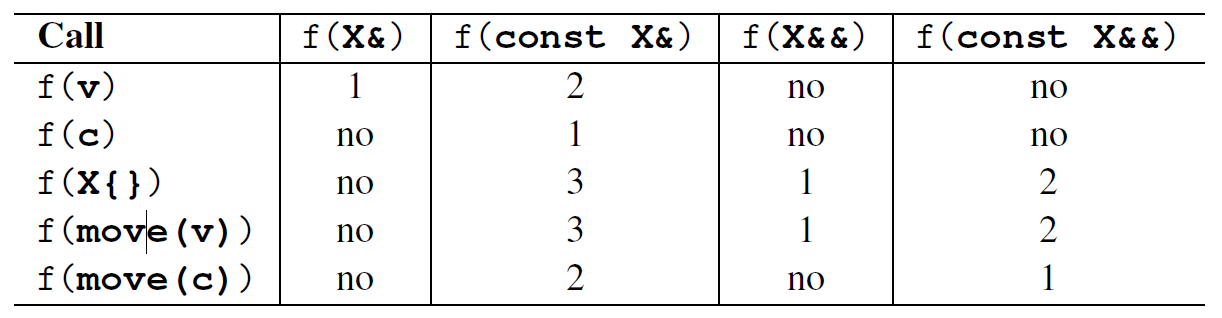
\includegraphics[width=0.8\textwidth]{content/1/chapter8/images/3}
\end{center}

\begin{itemize}
	\item 非\textit{const} lvalue引用只接受非\textit{const} lvalue。 
	\item rvalue引用只接受非\textit{const} rvalue。
	\item \textit{const} lvalue引用可以接受所有内容,并在没有提供其他重载的情况下充当备选机制。
\end{itemize}

下面是从表中提取的移动语义的备选机制规则:\par

\begin{center}
	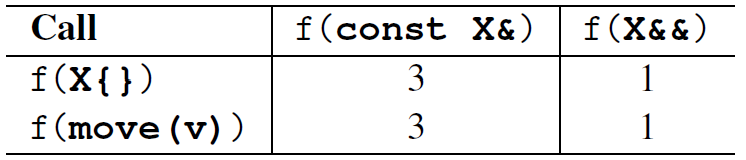
\includegraphics[width=0.6\textwidth]{content/1/chapter8/images/4}
\end{center}

如果向函数传递rvalue(临时对象或标记为\textit{std::move()}的对象),而移动语义没有特定的实现(通过接受rvalue引用声明),则使用通常的复制语义,\textit{const}\&接受实参。\par

请注意,在介绍通用引用/转发引用时会扩展此表。\par

有时可以将lvalue传递给rvalue引用(当使用模板形参时)。请注意,并非每个带有\&\&的声明都遵循相同的规则。这里的规则适用于使用\&\&声明类型(或类型别名)的情况。\par

\hspace*{\fill} \par %插入空行
\textbf{8.3.2 通过引用和值进行重载}

可以通过引用和值来声明函数:\par

\begin{lstlisting}[caption={}]
void f(X); // call-by-value
void f(const X&); // call-by-reference
void f(X&);
void f(X&&);
void f(const X&&);
\end{lstlisting}

原则上,这些重载的声明没问题。但是,按值调用和按引用调用之间没有特定的优先级。如果函数声明以值作为参数(它可以接受任何值类别的任何参数),那么任何匹配声明以引用作为参数都会造成歧义。\par

因此,只能通过值或引用(使用认为有用的尽可能多的引用重载)接受参数,但永远不要两者都接受。\par


































































